
% ***************************************************
% Example of an internal chapter
% ***************************************************
%This is an internal chapter of the thesis.
%If you have a long title, you can supply an abbreviated version to print in the Table of Contents using the optional argument to the \chapter command.
\chapter[Results]{Results and Discussion}
\label{Chap:label}	%CREATE YOUR OWN LABEL.
\pagestyle{headings}

This chapter aims to demonstrate the practicality and efficacy of the designed hardware. Performance metrics such as latency, resource utilisation, timing, and power consumption are analysed to gauge the design's effectiveness. The design is also tested with a small sample of real life packets of different properties to ensure the packet filter can correctly block unwanted packets. Preexisting solutions are then compared with the design, providing insight into the design's relative strength and weaknesses in areas of latency, power and thermal performance.



\section{Latency Performance}

Reducing the latency of hardware packet filtering in embedded systems is one of the key objectives of this thesis. As such, verification of the latency added due to the filtering is essential.

\subsection{Theoretical analysis}
The design employs a 200-stage shift register to temporarily store the incoming packet with each stage being 2bits wide. Given a clock frequency of 50Mhz, the added latency can be calculated to be $200 \times \frac{1}{50\times 10^6} = 4 \times 10^{-6} = 4\mu s$.

\subsection{Measured analysis}


The packet classifier's performance was measured with an Agilent MSO6054A MSO due to its high sampling rate of 4GSa/s. A PMOD pin was connected to output of an xor operation between the carrier sense line (crs\_dv) from the PHY and the crs\_dv post packet filtering. 

This process allowed the added latency to be measured characterised by the time between the rising and falling edge of either pulse as shown in figure \ref{fig:pf_added_latency}. The measured output can be seen to match the theoretical calculation of $4\mu s$.


\begin{figure}[h!]
    \centering
    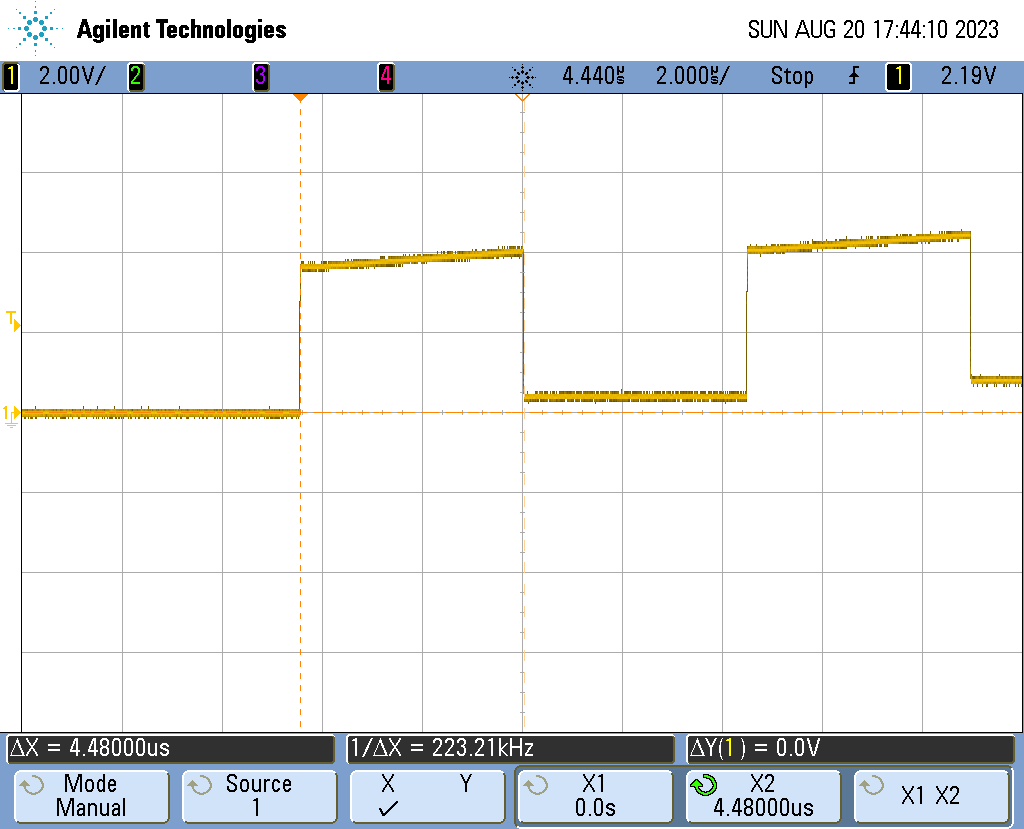
\includegraphics[width=0.75\textwidth]{Images/scope_4.png}
    \caption[Added latency by packet filter waveform]{Added latency by packet filter waveform.}
    \label{fig:pf_added_latency}
\end{figure}


The two distinct pulses are a result of the phase shift between the PHY crs\_dv and the delayed crs\_dv line. Additionally, the distance between the two pulses indicates the size of the packet. 


\subsection{Improvements}
A potential improvement on the design could be to integrate the packet classifier with the Ethernet MAC. This could reduce the added latency to zero by removing the need to store the packet in the additional shift register. The approach would involve storing the incoming packet and if the packet is later deemed to be blocked, the controlling FSM could be reset to ignore the packet. 











\section{Utilisation}

Resource utilisation is an integral part in validating the feasibility of implementing the design on a particular FPGA or microchip. This section details the post synthesis resource utilisation of the design on the Nexys A7-100T FPGA using Xilinx Vivado 2022.2. Namely, the NEORV32, Ethernet hardware and packet filter are analysed.


The resource breakdown referred to in this section can be found in figure \ref{fig:resource_util} while a more detailed breakdown of the resource utilisation including the primitives can be found in appendix \ref{app:res_usage}. 

\begin{figure}[h]
    \centering
    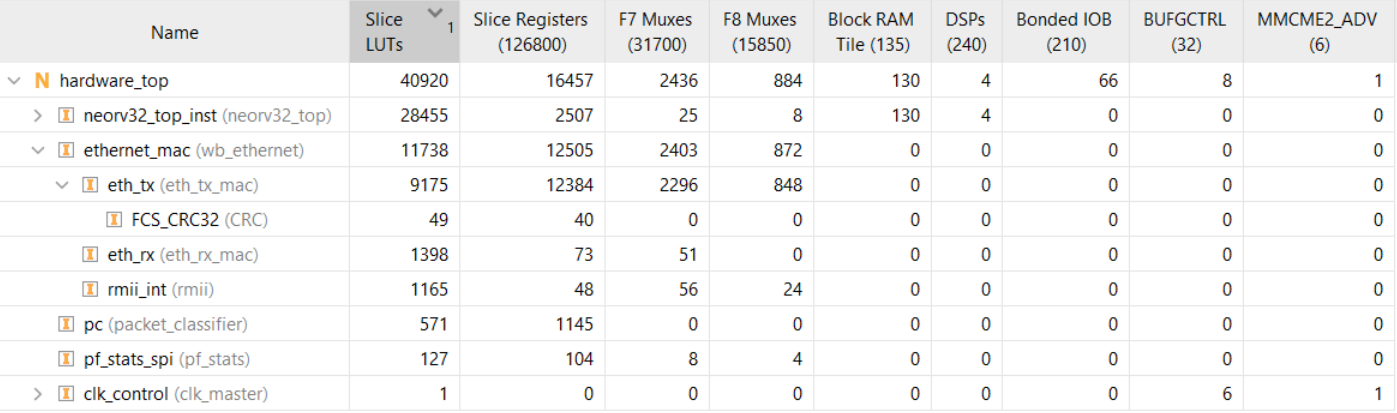
\includegraphics[width=1\textwidth]{Images/FPGAUtilisationResources.png}
    \caption[Summary of the resource utilisation on XC7A100T FPGA]{Summary of the resource utilisation on XC7A100T FPGA.}
    \label{fig:resource_util}
\end{figure}

 
The design as a whole uses a total of 64.5\% of the available slice LUTs, 12.9\% of the available flip flops and 96.3\% of the available BRAM.




\subsection{NEORV32 processor}

Significant LUT usage was attributed to the 32-bit wide wishbone interface. Considerable LUT consumption relates to frame buffers used in Ethernet hardware, elucidated further in subsection \ref{sec:eth_hardware_util}.


The NEORV32 SoC consumed the majority (69.5\%, or 28455), of the slice LUTs in the design. While many interfaces were enabled such as SPI, UART, GPIO, external interupts (XIRQ) and the true random number generator, a considerable amount of the LUTs were consumed by the 32bit wide wishbone interface. More specifically, 25992 slice LUTs, or 91.3\% of the NEORV32 usage. 

The large LUT utilisation relates to the frame buffers used in the Ethernet hardware, elucidated further in section \ref{sec:eth_hardware_util}. 

DSP48 blocks were also used by the SoC to handle the multiply operations to free up LUTs. 

The instruction memory (IMEM) and data memory (DMEM) sizes were configured to optimise the remaining BRAM blocks for increasing flexibility in firmware. Specifically, IMEM was allocated 256KB while the DMEM (acting as RAM) amounting to 168KB. 





\subsection{Ethernet hardware}
\label{sec:eth_hardware_util}


Comparatively, the Ethernet hardware accounted for 11738 slice LUTs and 12505 slice registers, most of which is consumed by the transmit logic (78\% LUT and 99\% registers). The considerable LUT utilisation in the transmit logic and NEORV32 Wishbone interface is due to the manner in which the frame buffer is written to. The complex operations such as address validation and array modification for writing to the frame buffer can be seen in listing \ref{lst:code_snippet}. Notably, the address validation specifically implements a 32bit wide comparator and the need to write/modify to the frame buffer array causes large LUT utilisation.

\begin{lstlisting}[style=vhdl, caption={Code for writing to the frame buffer}, label=lst:code_snippet]
if wb_i_addr >= x"13371004" and wb_i_addr <= x"13376410" then         
    -- Subtract 4100 from the address to get the virtual address
    virtAddr := to_integer((unsigned(wb_i_addr(15 downto 0)) - 4100));
    FRAME_BUFFER(8 + virtAddr) := wb_i_dat(31 downto 24);
    FRAME_BUFFER(9 + virtAddr) := wb_i_dat(23 downto 16);
    FRAME_BUFFER(10 + virtAddr) := wb_i_dat(15 downto 8);
    FRAME_BUFFER(11 + virtAddr) := wb_i_dat(7 downto 0);
end if;
\end{lstlisting}

This design choice also influenced the critical path delay as detailed further in section \ref{sec:timing_summary}. Optimisations to this area would be imperative to drastically reduce the resource consumption and improve the critical path delay.

By contrast, the receive logic consumed far less resources of 12\% of the Ethernet MAC's LUTs and only 1\% of the registers. This is attributed to the simpler design which stores the incoming packets with the correct endianness in the frame buffer before subsequently triggering an interrupt upon the packet's arrival. 

The rmii\_init logic acts as the glue logic between the PHY and the MAC. It facilitates the clock and bus domain crossings between the 8bit wide 80Mhz MAC and the 2bit wide 50Mhz RMII PHY. 



\subsection{Packet filter}

The packet classifier consumed a total of 571 slice LUTs and 1145 slice registers, suggesting a potential to increase the number of rules. Though, the fan-in and fan-out will likely need to be considered due to the nature of the implementation. The synthesiser's decision to use registers over BRAM for rule storage is likely due to the rules being small in size and that the BRAM blocks are better used elsewhere.

Alternatively, the minimal resource utilisation indicates that the design is suitable for implementation on smaller FPGAs or ASIC designs and will have negligible impact on the overall silicon area.





\section{Timing Summary}
\label{sec:timing_summary}


Timing analysis of the design provides insight into the critical path delay and the maximum frequency of the design. Basic results are presented in this section and are primarily around the Wishbone interface due to its role in the critical path. Importantly, the Wishbone interface operates at the same clock frequency as the NEORV32 processor which directly impacts the speed of the CPU for software based operations.

Initially, a single 50Mhz clock sourced from the onboard MMCM was used. A post-synthesis analysis indicated a positive slack in the design, allowing for the clock frequency to be updated to 80Mhz. This was done to increase the performance of the CPU so that it could process network packets faster in software.

After resynthesising, a worst negative slack for setup time of -2.634ns was reported with a total of 82 endpoints failing the constraints. Additionally, a worst hold slack of -0.021ns was reported. The identified critical path originates from the Wishbone interface to the BRAM block within the Ethernet hardware, shown in figure \ref{fig:crit_path}. Due to the NEORV32's implementation of the Wishbone bus, the critical path cannot be easily improved and is the leading limitation in the speed of the design. 


\begin{figure}[h]
    \centering
    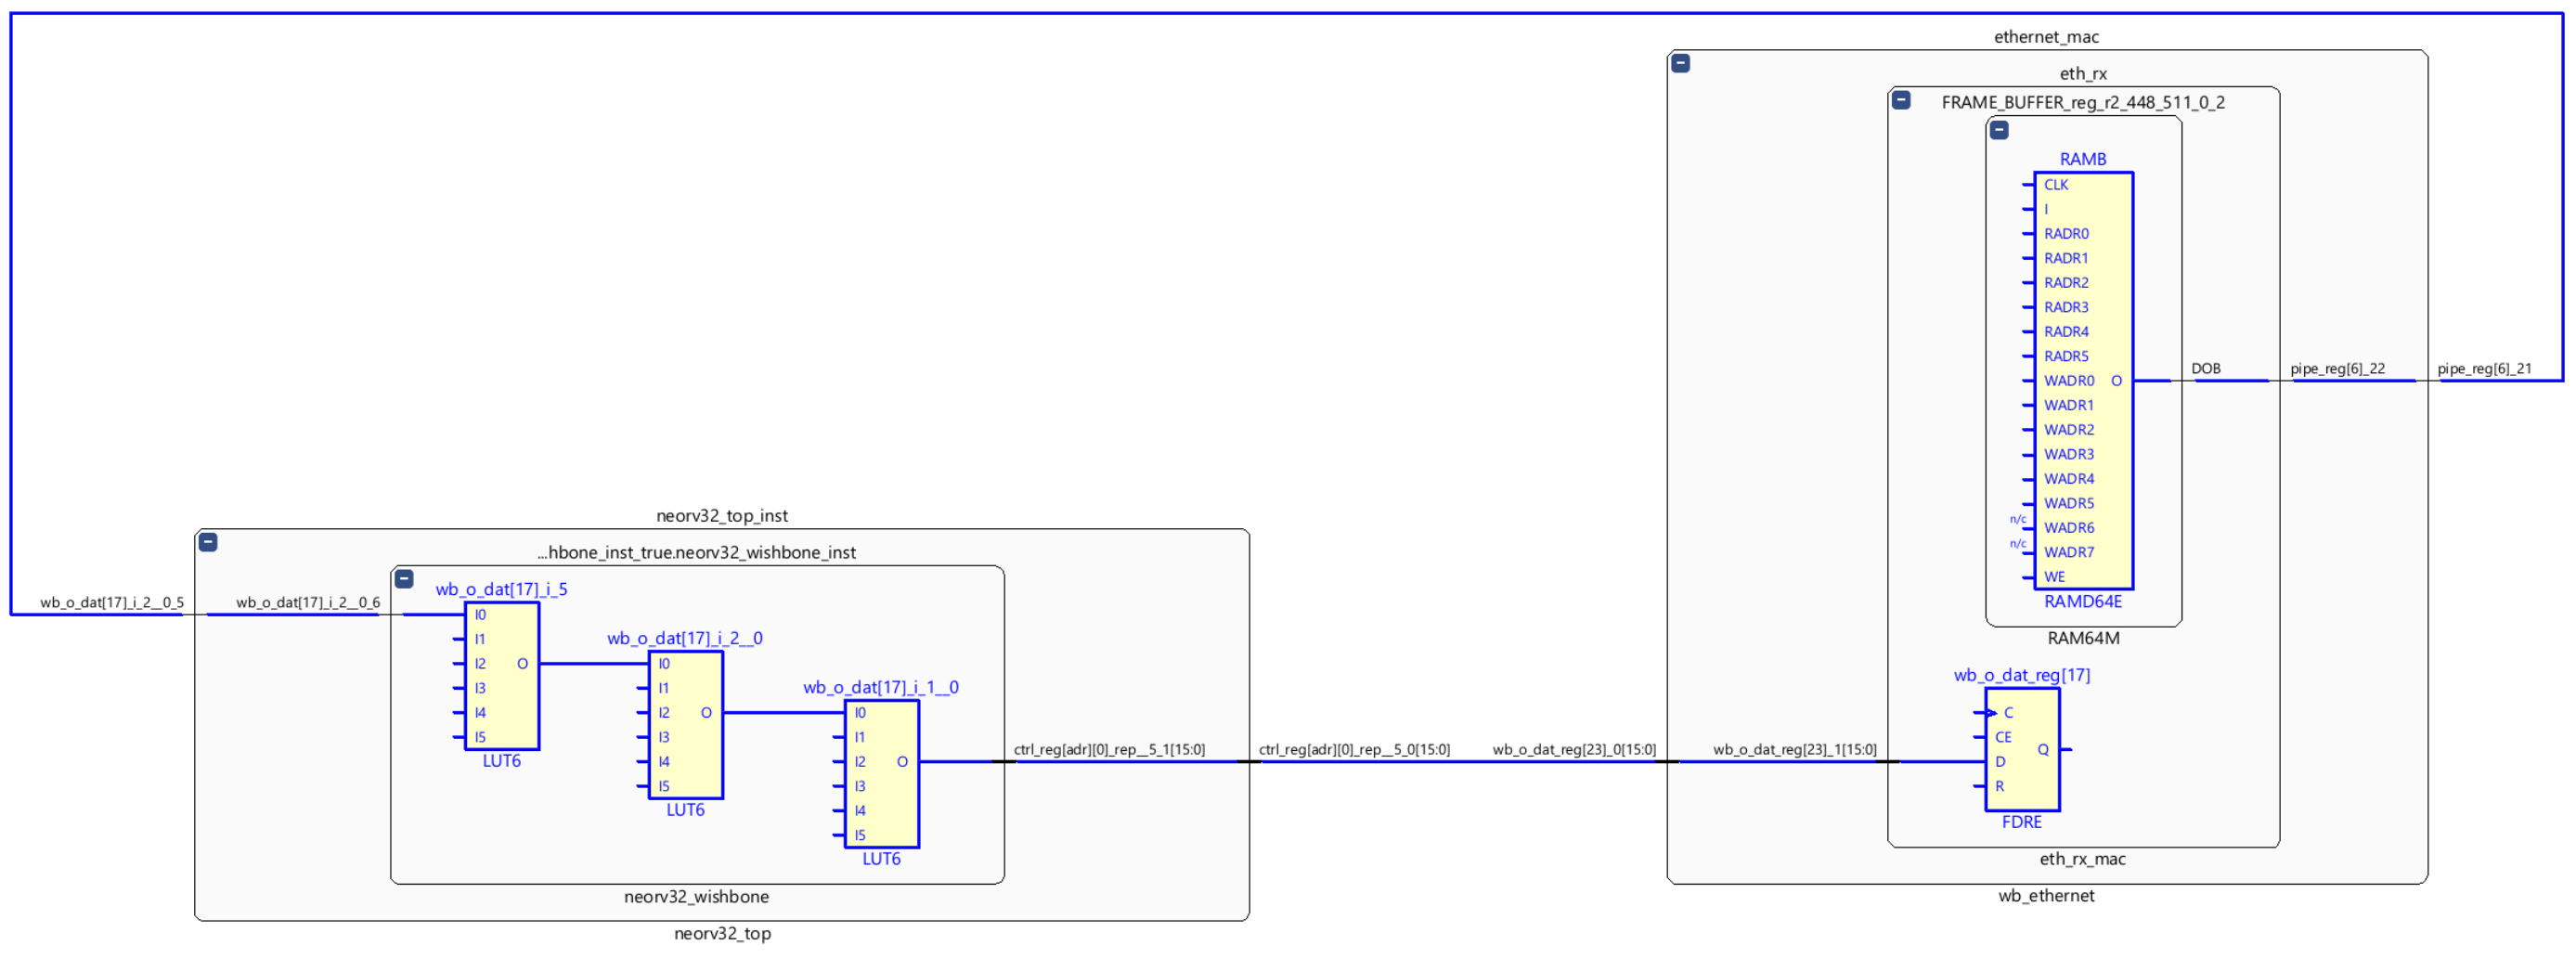
\includegraphics[width=1\textwidth]{Images/critical_path_delay_schematic.png}
    \caption[Critical path in SoC design]{Critical path in SoC design.}
    \label{fig:crit_path}
\end{figure}


While in practice these timing constraints do not crucially impact the design's operation, caution is advised in future adaptations or usage. Other paths were also encroaching on a slack of zero and hence the design was limited to 80Mhz. Testing at 90Mhz was conducted, however, the design was found to be unstable and had a large increase in the number of failing endpoints.

More accurate timing constraints would need to be set to acquire the absolute maximum frequency of the design. Though, this was outside the scope of this thesis. 





















\section{Filtering performance}

Blocking unwanted packets is imperative to a firewall's operation with any packets bypassing the filter rendering it useless. Testing all possible permutations of bits going through the firewall is infeasible due to the sheer number of packets needed, which is on the order of $2^{104}$. For example, a complete testing suite for all source IP addresses alone would require $2^{32}$ (about 4.3 billion) packets to be sent to the device. Therefore, a small sample of packets, shown in table \ref{tab:firewall_testing_config}, were tested to ensure the filter is working as intended. 


\subsection{Test setup}

Four hosts distributed across two networks were used to test the device as depicted in the network diagram in figure \ref{fig:network_layout_test}. The network consisted of three Raspberry Pi 4s and an x86 based Ubuntu machine. The specifics characteristics of these devices are irrelevant to this thesis, given that they all adhere to the TCP/IP standards. More specifically they were chosen due to their capability to run Python scripts and are accessibility over Ethernet. A common script\footnote[1]{The Python \textit{test} script can be found at https://github.com/matty0005/thesis-tools} was used on all devices to test each of the services available on different ports and protocols. 



\begin{figure}[h]
    \centering
    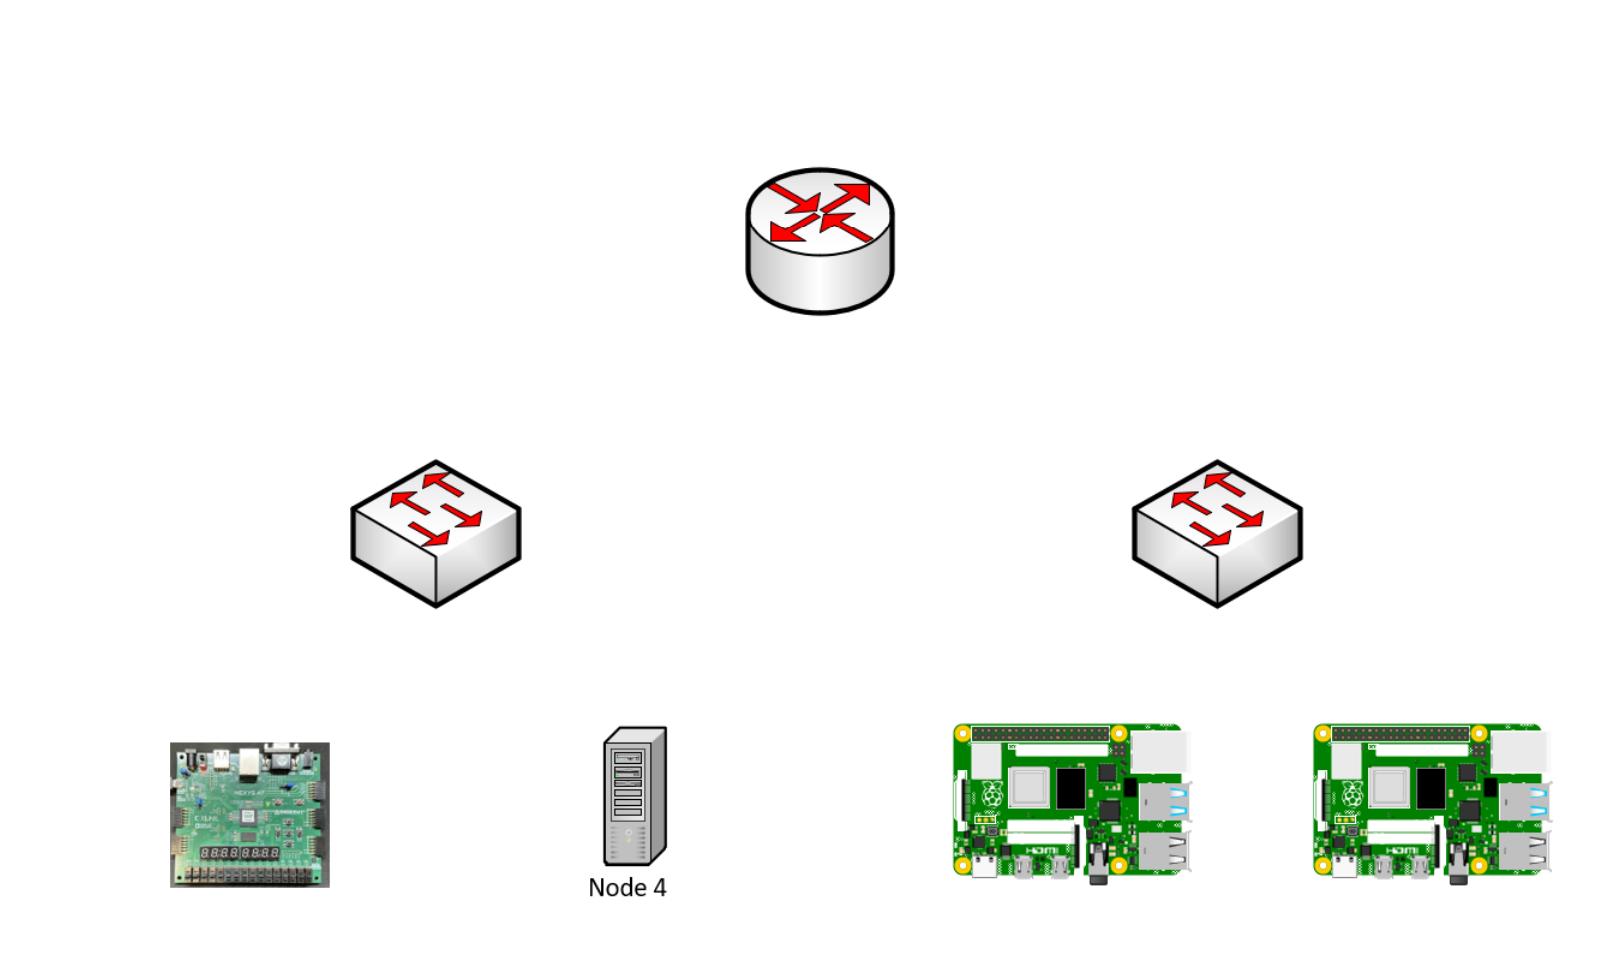
\includegraphics[width=1\textwidth]{Images/NetworkArchitecture.png}
    \caption[Network architecture for firewall tests]{Network architecture for firewall tests.}
    \label{fig:network_layout_test}
\end{figure}

\newpage

The rules shown in table \ref{tab:firewall_testing_config} shows the rules that were loaded on the packet filter.  While these test cases is only a subset of the total coverage, a mix of different combinations of ports, protocols and IP addresses were chosen. More specifically the rules were chosen to test the following cases:



\begin{itemize}
    \item All devices can access the device in some way (eg, over ICMP),
    \item All machines could access at least two services,
    \item Identical ports over different protocols can be filtered (eg, port 1337 over TCP and UDP),
    \item Ports can be blocked on a device even though the device can access other services with the same protocol,
    \item The wildcard operator works in each field, and
    \item Any port that is not explicitly allowed is blocked.
\end{itemize}

By default, as the packet filter is a default-deny, any packet that doesn't fit these constraints is blocked and can be verified in the tests summarised in \ref{tab:firewall_test_cases}.


\begin{table}[h!]
    \centering
    \caption{Firewall configuration for testing}
    \label{tab:firewall_testing_config}
    \begin{tabular}{ccccc}
        \toprule
        Source IP & Destination IP & Source Port & Destination Port & Protocol \\
        \midrule
        any       & 10.20.1.34      & n/a         & n/a              & ICMP     \\
        10.0.0.5  & 10.20.1.34      & any         & any              & UDP      \\
        10.0.0.5  & 10.20.1.34      & any         & 80               & TCP      \\
        10.0.0.93 & 10.20.1.34      & any         & 1337             & TCP      \\
        10.0.0.93 & 10.20.1.34      & any         & 9999             & UDP      \\
        10.20.1.10& 10.20.1.34      & any         & 1337             & any      \\
        10.20.1.10& 10.20.1.34      & any         & any              & UDP      \\
        10.20.1.11& 10.20.1.34      & any         & 9999             & UDP      \\
        \bottomrule
    \end{tabular}
    
\end{table}

Typically, firewalls have a second interface that connects to a local network, allowing packets from multiple IP addresses to be processed and forwarded on. However, in this setup, a single device is behind the firewall, requiring the \textit{destination IP's} to be the same (the NEORV32's IP address, 10.20.1.34). 

Additionally, the \textit{source port} was configured to allow any source port through. This is important due to the client arbitrarily choosing the source port at random. Therefore, a wildcard was used as this makes the source port impossible to predict. It's worth noting that some niche programs operate with predicable ports, though none of the programs used in this test were of this nature.


\subsection{Test results}

A summary of the results can be seen in table \ref{tab:firewall_test_cases} which show the firewall blocking and allowing the respective packets correctly.

\begin{table}[h]
    \centering
    \caption{Summary of packets including expected and actual outcomes}
    \label{tab:firewall_test_cases}
    \begin{tabular}{m{2.25cm}m{2cm}m{1.5cm}m{2cm}m{2cm}m{2cm}m{2cm}}
        \toprule
        Device & Dest. IP & Protocol & Src. Port & Dest. Port & Expected Outcome & Actual Outcome \\
        \midrule
        \parbox[c]{2.25cm}{\centering Node1\\\textcolor{gray}{(10.20.1.10)} \vspace*{14pt}} & 10.20.1.34 & TCP & Any & 1337 & Allow & Allowed \\
        \parbox[c]{2.25cm}{\centering Node2\\\textcolor{gray}{(10.20.1.11)} \vspace*{14pt}} & 10.20.1.34 & ICMP & - & - & Allow & Allowed \\
        \parbox[c]{2.25cm}{\centering Node3\\\textcolor{gray}{(10.0.0.5)} \vspace*{14pt}} & 10.20.1.34 & UDP & Any & 9999 & Allow & Allowed \\
        \parbox[c]{2.25cm}{\centering Node4\\\textcolor{gray}{(10.0.0.93)} \vspace*{14pt}} & 10.20.1.34 & TCP & Any & 1337 & Allow & Allowed \\
        \parbox[c]{2.25cm}{\centering Node1\\\textcolor{gray}{(10.20.1.10)} \vspace*{14pt}} & 10.20.1.34 & UDP & Any & 1337 & Allow & Allowed \\
        \parbox[c]{2.25cm}{\centering Node3\\\textcolor{gray}{(10.0.0.5)} \vspace*{14pt}} & 10.20.1.34 & TCP & Any & 80 & Allow & Allowed \\
        \parbox[c]{2.25cm}{\centering Node3\\\textcolor{gray}{(10.0.0.5)} \vspace*{14pt}} & 10.20.1.34 & TCP & Any & 1337 & Deny & Denied \\
        \parbox[c]{2.25cm}{\centering Node2\\\textcolor{gray}{(10.20.1.11)} \vspace*{14pt}} & 10.20.1.34 & TCP & Any & 1337 & Deny & Denied \\
        \parbox[c]{2.25cm}{\centering Node4\\\textcolor{gray}{(10.0.0.93)} \vspace*{14pt}} & 10.20.1.34 & UDP & Any & 1337 & Deny & Denied \\
        \parbox[c]{2.25cm}{\centering Node4\\\textcolor{gray}{(10.0.0.93)} \vspace*{14pt}} & 10.20.1.34 & TCP & Any & 80 & Deny & Denied \\
        \bottomrule
    \end{tabular}
    
\end{table}


The detailed output from the script on each host is available in appendix \ref{app:testing_pf}. While these tests don't formally prove the firewall is correctly working, they do provide substantial evidence of the design's correctness. It's important to note that additional rigorous testing, which wasn't formally documented, was conducted throughout the development of the design. Such an example test case involves spamming ping packets from one host while sending valid packets from another. 

These results stipulate the devices suitability for use in a real world environment. The filter exhibits capacity to filter out the significant majority of unwanted packets, making it ideal for low security applications. However, formal verification and meticulous testing is imperative to suitability for high-security applications. With the absence of these in the above tests, the design would necessitate further validation to be deployed in high security environments. 















\section{Comparison to preexisting solutions}

To ensure the effectiveness of the designed hardware, comparisons to preexisting solutions with \textit{Fast Ethernet} (100Mbits/s) were conducted. The selected devices include the WIZ5500 Pico \footnote[1]{See: https://www.wiznet.io/product-item/w5500-evb-pico/}, Nucleo-F767ZI \footnote[2]{See: https://www.st.com/en/evaluation-tools/nucleo-f767zi.html} and MilkV-Duo \footnote[3]{See: https://milkv.io/duo}.

The WIZ5500 Pico integrates a \textit{Raspberry Pi RP2040} (ARM-based) as its MCU, operating at 133Mhz, and employs the \textit{WIZ5500} IC to manage Ethernet traffic. Notably, the WIZ5500 handles layers one to four onboard and interfaces ov er SPI. This is in contrast to the other designs compared which use an external PHY and then have the higher layers in software. 

The Nucleo-F767ZI (referred to as just F767ZI) is powered by the \textit{STM32F767} (ARM-based) MCU and features an onboard \textit{LAN8742A} PHY chip. Similarly to the Nexys A7 board, the LAN8742A PHY chip connects to the STM32F767 over RMII and has hardware support for. This establishes a good comparison between the two devices from a hardware perspective. However, unlike the Nexys A7, it utilised the LwIP network stack opposed to FreeRTOS-Plus-TCP. 


The most contemporary board in the lineup is the MilkV-Duo which employs the 64-bit RISC-V \textit{CVITEK CV1800B} processor. Operating at 1Ghz, the dual-core processor includes 64MB of RAM and incorporates an Ethernet MAC and PHY directly within the same package. The MilkV runs vanilla Linux on the first core and FreeRTOS on the second. Throughout these tests, Linux was used as it had greater support at the time of testing. 

The following sections detail the relative performance of the respective devices in terms of latency, throughput, security and power consumption. Thermal measurements are also conducted to bring greater detail to the power consumption of the devices.


\newpage

\subsection{Network latency tests}


A simply UDP ping program was devised on each device to empirically assess the round-trip-time (RTT). This not only helps understand the latency of the system as a while, but by using two different packet sizes, the software overhead can be assessed. The program was configured to receive a UDP packet on port 9999 and reply with a corresponding packet. 

To alleviate nuances in the network and once off delays, 1,000 UDP packets were averaged and the results are presented in \ref{fig:avg_udp_rtt}. A table highlighting the numerical values of the results can be found in appendix \ref{app:udp_ping_measurements}.

Two specific UDP payloads sizes, 8 bytes and 256 bytes, were selected to evaluate the software overhead. 

These values were chosen due to the additional time required to process the packet in hardware is in the order of nanoseconds. More specifically, the delay can be calculated by knowing the bitrate and difference in packet size. In this test, at a speed of 100Mbit/s, sending 248 more bytes takes an additional $\frac{248 \times 8}{100 \times 10^6}=19.84\mu s$. In contrast, software processing time scales up significantly with the packet size, due to additional data manipulation and processing

\begin{figure}[ht]
    \centering
    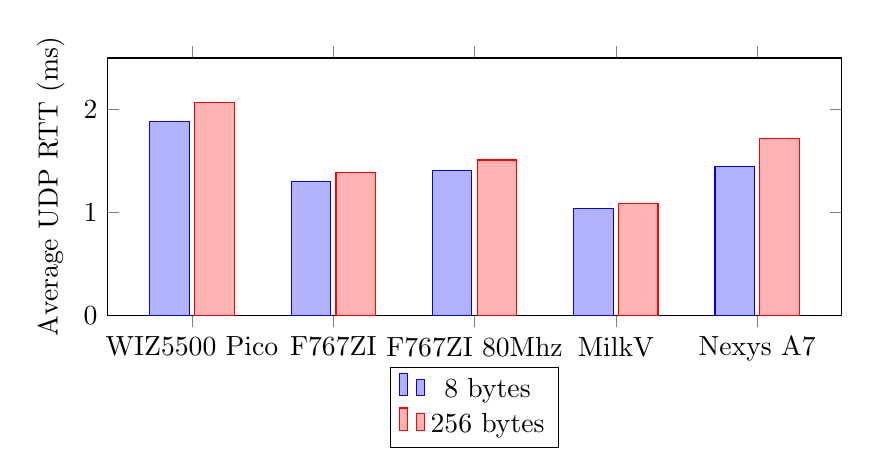
\begin{tikzpicture}
    \begin{axis}[
        ybar,
        symbolic x coords={WIZ5500 Pico, F767ZI, F767ZI 80Mhz, MilkV, Nexys A7},
        xtick=data,
        ylabel={Average UDP RTT (ms)},
        legend style={at={(0.5,-0.2)},anchor=north},
        enlarge x limits=0.15,
        ymin=0,
        ymax=2.5,
        width=0.9\textwidth,
        height=0.4\textwidth,
        bar width=0.5cm
    ]
    \addplot coordinates {
        (WIZ5500 Pico,1.88)
        (F767ZI 80Mhz,1.41)
        (F767ZI,1.30)
        (Nexys A7,1.45)
        (MilkV,1.04)
    };
    \addplot coordinates {
        (WIZ5500 Pico,2.07)
        (F767ZI 80Mhz,1.51)
        (F767ZI,1.39)
        (Nexys A7,1.72)
        (MilkV,1.09)
    };
    \legend{8 bytes,256 bytes}
    \end{axis}
    \end{tikzpicture}
    \caption{Average UDP RTT for different devices and payload sizes.}
    \label{fig:avg_udp_rtt}
    \end{figure}
    

Testing on the Nexys A7 resulted a larger difference compared to the competing products and indicates a larger software overhead. It is hypothesised that this is a consequence if the FreeRTOS-Plus-TCP stack, which likely requires more computations per packet than LwIP on the F767ZI. Two tests on the F767ZI was conducted to understand the effect of clock frequency, one at the default 96Mhz and another at 80Mhz to match the Nexys A7. The results indicated a small improvement in latency of 0.11ms when using 96Mhz clock speed on the F767ZI. A decrease in latency is expected on the Nexys A7 if the clock frequency can be increased. This is further supported with the MilkV Duo which runs at 1Ghz and has a lower latency than both the F767ZI and Nexys A7.

The results from this section support the design given in this thesis is comparable to preexisting solutions in terms of overall latency. However, latency is not the only metric used in assessing network performance. Network throughput is another imperative metric and is discussed in the next section.


\subsection{Network throughput tests}
This section primarily focuses on the throughput tests amount the F767ZI, MilkV Duo and Nexys A7 boards. The WIZ5500 Pico was exempt from testing due to a lack of support for Iperf 3, a universally accepted tool for bandwidth testing between two devices. Both FreeRTOS and LwIP have Iperf 3 server implementations which were used to test the throughput of the devices.


The client device, an x86-based desktop machine, was connected to the network at gigabit speeds, ensuring there was no bottleneck on the client side. Test results were averaged over ten runs to ensure accuracy and account for any anomalies. Table \ref{tab:bitrate_tests} summaries the bitrates of the tested devices. The detailed Iperf 3 outputs from each test can be found in appendix \ref{app:iperf3_test_results}.


\begin{table}[h]
    \centering
    \caption{Bitrate of various embedded devices}
    \label{tab:bitrate_tests}
    \begin{tabular}{P{3.5cm} P{3.5cm}}
        \toprule
        Device & Bitrate \\
        \midrule

        Nexys A7 & 1.32Mbits/s \\
        F767ZI & 7.11Mbits/s \\
        MilkV & 92.4Mbits/s \\
        \bottomrule
    \end{tabular}
    
\end{table}



The MilkV Duo with the 1Ghz processor, saturated the 100Mbit/s \textit{Fast Ethernet} interface, aligning with expectations. The test is consistent with the hypothesis that software constraints bottleneck the Nexys A7's performance. It is also believed that suboptimal task priorities and interrupt configurations in FreeRTOS are contributing to this limitation, as demonstrated by the dip in performance when the tick frequency in FreeRTOS was altered from 500Hz to 1000Hz, causing a notable 41.8\% reduction in performance. This would make the scheduler interrupt the tasks more frequently and hence give less time for the packet to be processed before switching tasks.

The F767ZI showcased a superior throughput over the Nexys A7, attributed primarily to the utilisation of LwIP over FreeRTOS-Plus-TCP and having more refined drivers with better interrupt handling and task scheduling.

While the Nexys A7 provides comparable performance in the UDP ping tests, the throughput is lacking and provides an opportunity for improvement in the firmware. Despite this, the Nexys A7, which employs a hardware firewall, holds an advantage in terms of security, which is discussed in the next section.


\subsection{Security analysis}

The distinctive feature of the design on the Nexys A7, developed in this thesis, is the incorporation of a hardware packet filter, whereas the other devices rely on software-based packet filters. This hardware approach benefits from intrinsic robustness against particular vulnerabilities typically found within embedded systems, such as power-glitch attacks (also commonly referred to as fault-injection).

Power-glitch attacks, while hard to execute in a real world situation, provide a threat to embedded systems, characterised by rapid power off-and-on cycles at critical sections aimed at bypassing specific code instructions. Although in practice, these attacks are extremely rare, it does provide an advantage to the hardware firewall in system security and robustness.

The design in this thesis operates by directly interfacing and processing the bits with the PHY which makes it less susceptible to power-glitch attacks. This is due to comparison logic being independent of the CPU and not consisting of a set of instructions, but rather a set of dedicated logic which is more resilient. Furthermore, the attack surface (a group of potential vulnerabilities accessible to a malicious actor) of the design is much smaller due to much fewer known hardware vulnerabilities. It is worth noting that exhaustive formal verification would be necessary to ensure the design is secure against power-glitch attacks. However, this was outside the scope of this thesis.


As discussed earlier in this thesis, a benefit of hardware packet filters is the latency performance. Consequently, the firewall latency was compared with preexisting software solutions in the next section.


\subsection{Firewall latency}

To accurately gauge the latency introduced by software firewalls, a GPIO pin was configured to toggle states, marking the entry and exit of a packet during the filtering process. This approach makes the assumption that the latency involved in setting the GPIO pin states is reciprocal and the turn on and turn of time is the same, thereby minimising the potential influence on the overall delay measurement.

For consistency and to ensure a level playing field in the comparisons, the software based implementation of the firewall on the Nucleo-F767ZI board used eight rules. This aligns with the FPGA design's limitation and ensures the analysis remains fair.

Utilising an oscilloscope enabled precise time measurements of the firewall latency as found in figure \ref{fig:sw_pf_timings}. These measurements revealed the timings are dependent on the quantity and the positioning of the applied rules. For example, the best case scenario is when the first rule is matched, resulting in a lower latency, whereas the worst case is when the last rule is matched, resulting in a higher latency.

A best case time was measured to be $3.14\mu s$ (figure \ref{fig:sw_pf_best_case}) while an average case was $10.76\mu s$ (figure \ref{fig:sw_pf_bad_case}).


\begin{figure}[h]
    \centering
    \begin{subfigure}[b]{0.45\textwidth} % Adjust the width to your needs
        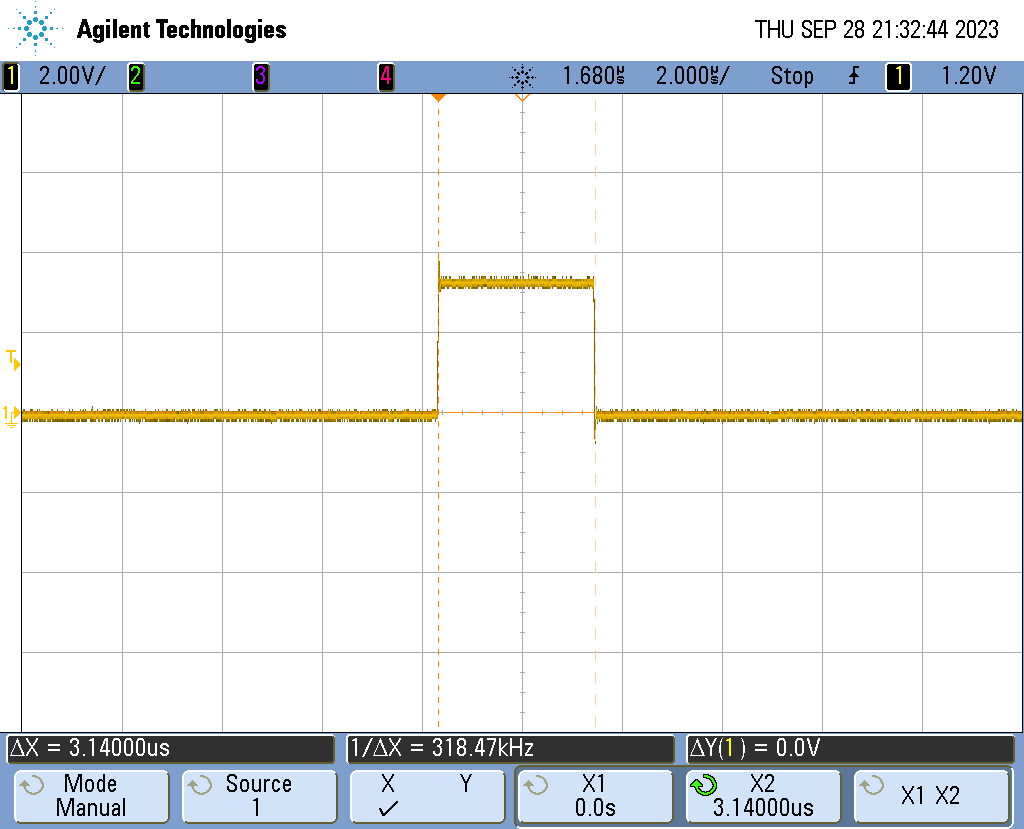
\includegraphics[width=\textwidth]{Images/sw_pf_best_case.png}
        \caption{Best case scenario}
        \label{fig:sw_pf_best_case}
    \end{subfigure}
    \hfill % this will add a small space between the two images
    \begin{subfigure}[b]{0.45\textwidth} % Adjust the width to your needs
        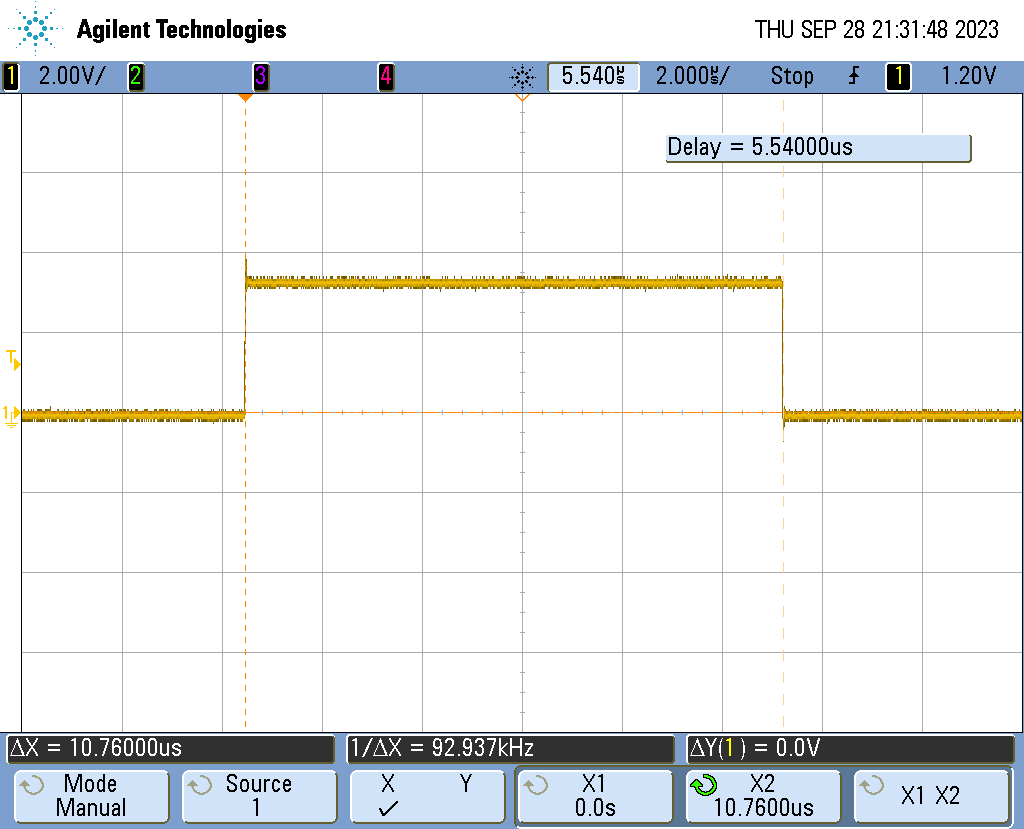
\includegraphics[width=\textwidth]{Images/sw_pf_bad_case.png}
        \caption{Average case}
        \label{fig:sw_pf_bad_case}
    \end{subfigure}
    \caption{Software packet classifier timings}
    \label{fig:sw_pf_timings}
\end{figure}


The lower latency observed in the ideal software scenario (figure \ref{fig:sw_pf_best_case}) is attributed to the packet matching the first rule, thereby reducing the necessary computations. This made the software filter quicker than the hardware filter in this case. However, in real-world applications, it is impractical to assume that the first rule will always be matched. Instead, the average-case latency is more indicative of actual performance.

It is important to recognise that these delays influence throughput as the processor is limited to only one task at a time and cannot multitask. 

In low bandwidth environments, there is little benefit, excluding their security advantage, to hardware firewalls in embedded systems. However, in scenarios where latency holds a significance, such as real-time robotic control systems, or where utmost security is imperative, as seen in secure access control systems, hardware firewalls provide as a more superior solution. Another difference between hardware and software implementations is the efficiency of the design, which will be detailed in the next section. 




\subsection{Power consumed between boards}

This section considers the power consumed between the four boards compared in this chapter. Detailed power analysis on the Nexys A7 board can be found in section \ref{sec:power_analysis}. The \textit{Nordic Semiconductor Power Profiler Kit 2} (PPK2) was used to measure the current consumption of the device over time. As all systems in these tests operate at 5V, only the current will be measured. A summary of the results can be found in figure \ref{fig:power_comparison}, while the data in tabular form can be found in appendix \ref{app:current_measurements}.

Each board underwent four different tests to measure current consumption: Idle, Busy, No Ethernet, and Clean State. In the \textit{Idle} measurement, the design is loaded but not processing any packets or computing anything. For the \textit{Busy} test, measurements were taken while the device actively received and processed packets. It should be noted that these values are typically lower than the Idle measurements, as the flashing status LED tends to impact the power consumption more than the hardware's power consumption. The \textit{No Ethernet} test refers to measurements taken when the device is idle with the Ethernet cable disconnected, showcasing the PHY chips' low-power sleep-like state in the absence of an Ethernet connection. Lastly, the \textit{Clean State} involves measuring the device while idling with no design loaded, effectively measuring the quiescent current of the device.



\begin{figure}[ht]
    \centering
    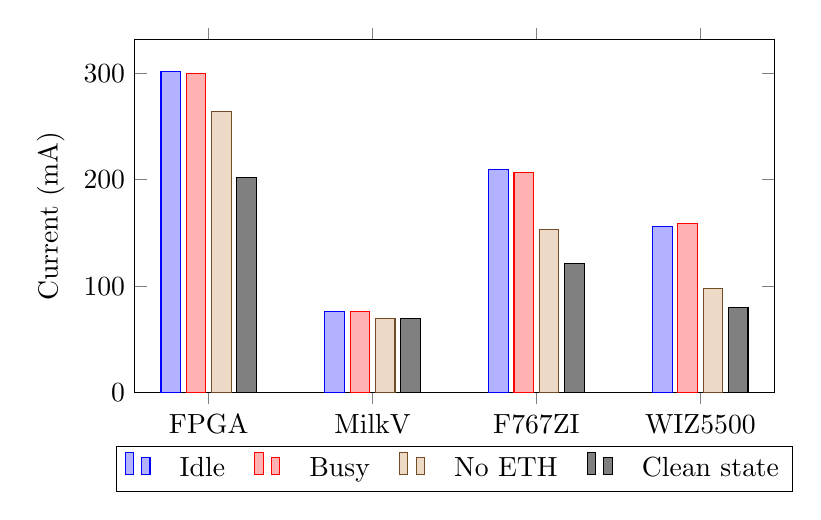
\begin{tikzpicture}
        \begin{axis}[
            ybar,
            bar width=0.25cm,
            width=0.8\textwidth,
            height=0.5\textwidth,
            enlarge x limits=0.15, % Adjusted value to make the bars closer
            ylabel={Current (mA)},
            symbolic x coords={FPGA, MilkV, F767ZI, WIZ5500},
            xtick=data,
            legend style={
                at={(0.5,-0.15)},
                anchor=north,
                legend columns=-1,
                legend cell align=left,
                legend image post style={scale=1}, % Adjust this value for spacing
                column sep=0.3cm % Adjust the space between each legend entry
            },
            legend cell align=left,
            ymin=0,
        ]
        \addplot coordinates {
            (FPGA, 301.4)
            (MilkV, 76.27)
            (F767ZI, 209.25)
            (WIZ5500, 155.88)
        };
        \addlegendentry{Idle}
        
        \addplot coordinates {
            (FPGA, 300.13)
            (MilkV, 76.53)
            (F767ZI, 206.9)
            (WIZ5500, 158.67)
        };
        \addlegendentry{Busy}
    
        \addplot coordinates {
            (FPGA, 264)
            (MilkV, 69.23)
            (F767ZI, 153.46)
            (WIZ5500, 97.9)
        };
        \addlegendentry{No ETH}

        % New data for "Complete Idle"
        \addplot coordinates {
            (FPGA, 202.13)
            (MilkV, 69.23)
            (F767ZI, 121.31)
            (WIZ5500, 80.35)
        };
        \addlegendentry{Clean state}

        \end{axis}
    \end{tikzpicture}
    \caption{Comparison of Idle, Busy, and No eth currents for devices}
    \label{fig:power_comparison}
    \end{figure}
    


Analysing figure \ref{fig:power_comparison} reveals the differences between the clean and busy states. The Nexys A7 board displayed the largest discrepancy, with a 99.27mA difference, compared to the 87.94mA difference observed in the F767ZI board. It's worth noting that the Nexys A7's clean state measurement was taken without the hardware design applied (Ethernet MAC, packet filter, and RISC-V core), resulting in a separate reading of 283.75mA when the design and hardware was loaded (excluding firmware). This indicates that, despite having the highest quiescent current, the Nexys A7 also exhibits the largest design current for the project. Power optimisations would be necessary in components such as the Ethernet and the RISC-V core to perform closer to preexisting solutions, although this was not a primary focus of this thesis.

All these tests were conducted without enabling a firewall. Additional tests were carried out to assess the Nexys A7 board's current consumption with the hardware firewall enabled and with a software firewall implemented on the F767ZI. No measurable differences were observed when the hardware packet filter was enabled or disabled, possibly attributed to the limited resolution of the measurement equipment. However, the software implementation resulted in a relative increase of 1mA due to the execution of more comparisons per packet.

Currently, the outcomes suggest that the Nexys A7 board might not be ideal for low-power applications due to its considerable quiescent current. The board is primarily intended for developmental purposes and not for power efficiency. In a production setting, a revised board design would omit unnecessary components and could incorporate more energy-efficient designs or FPGAs. While this falls outside the scope for this thesis, it is an important consideration for future work.

Moreover, current consumption naturally correlates with heat production of the device. By using a thermal camera, one can learn where the majority of the power is being drawn and as such is discussed in the next section.









\subsection{Thermal analysis}

A Flir One thermal camera was used to periodically record the temperatures of the boards and a summary of results is provided in table \ref{tab:temperature_comparison}. Throughout the examination, a constant ambient room temperature of $24.8\degree C$ was maintained. Measurements were taken at 5, 10, 30, 60 and 120 minute intervals to track the influence of the PCB board had on the thermal properties of the chips. This consideration is important as larger PCBs possess greater thermal mass which can distort the results and require time to get up-to temperature. Detailed results can be found in appendix \ref{app:thermal_measurements}. Since no substantial thermal variations were observed after 60 minutes, the tests was concluded at the 120-minute mark.


\begin{table}[h]
    \centering
    \caption{Temperature comparison of different chips during the test}
    \label{tab:temperature_comparison}
    \begin{tabular}{P{3.5cm} P{3.5cm} P{3.5cm} }
        \toprule
        Time & Chip & Temperature ($\degree C$) \\
        \midrule
        5 min & WIZ5500 & 58.0  \\
              & FPGA & 38.0 \\
              & MilkV & 36.7 \\
              & F767ZI & 35.9 \\
        \midrule
        2 hours & WIZ5500 & 56.8 \\
                & FPGA & 40.4 \\
                & MilkV & 38.1 \\
                & F767ZI & 36.8 \\
        \bottomrule
    \end{tabular}
\end{table}


Refer to figure \ref{fig:thermal_2hr} for a visual representation of each board's thermal distribution after two hours. It's important to consider these measurements as indicative rather than conclusive, highlighting the chips' relative temperatures and hotspots. This is because discrepancies are expected  due to the thermal camera's self-calibration process and the manual aiming of the camera to capture maximum heat being inherently inaccurate.


\begin{figure}[h]
    \centering
    \begin{subfigure}[b]{0.45\textwidth} % Adjust the width to your needs
        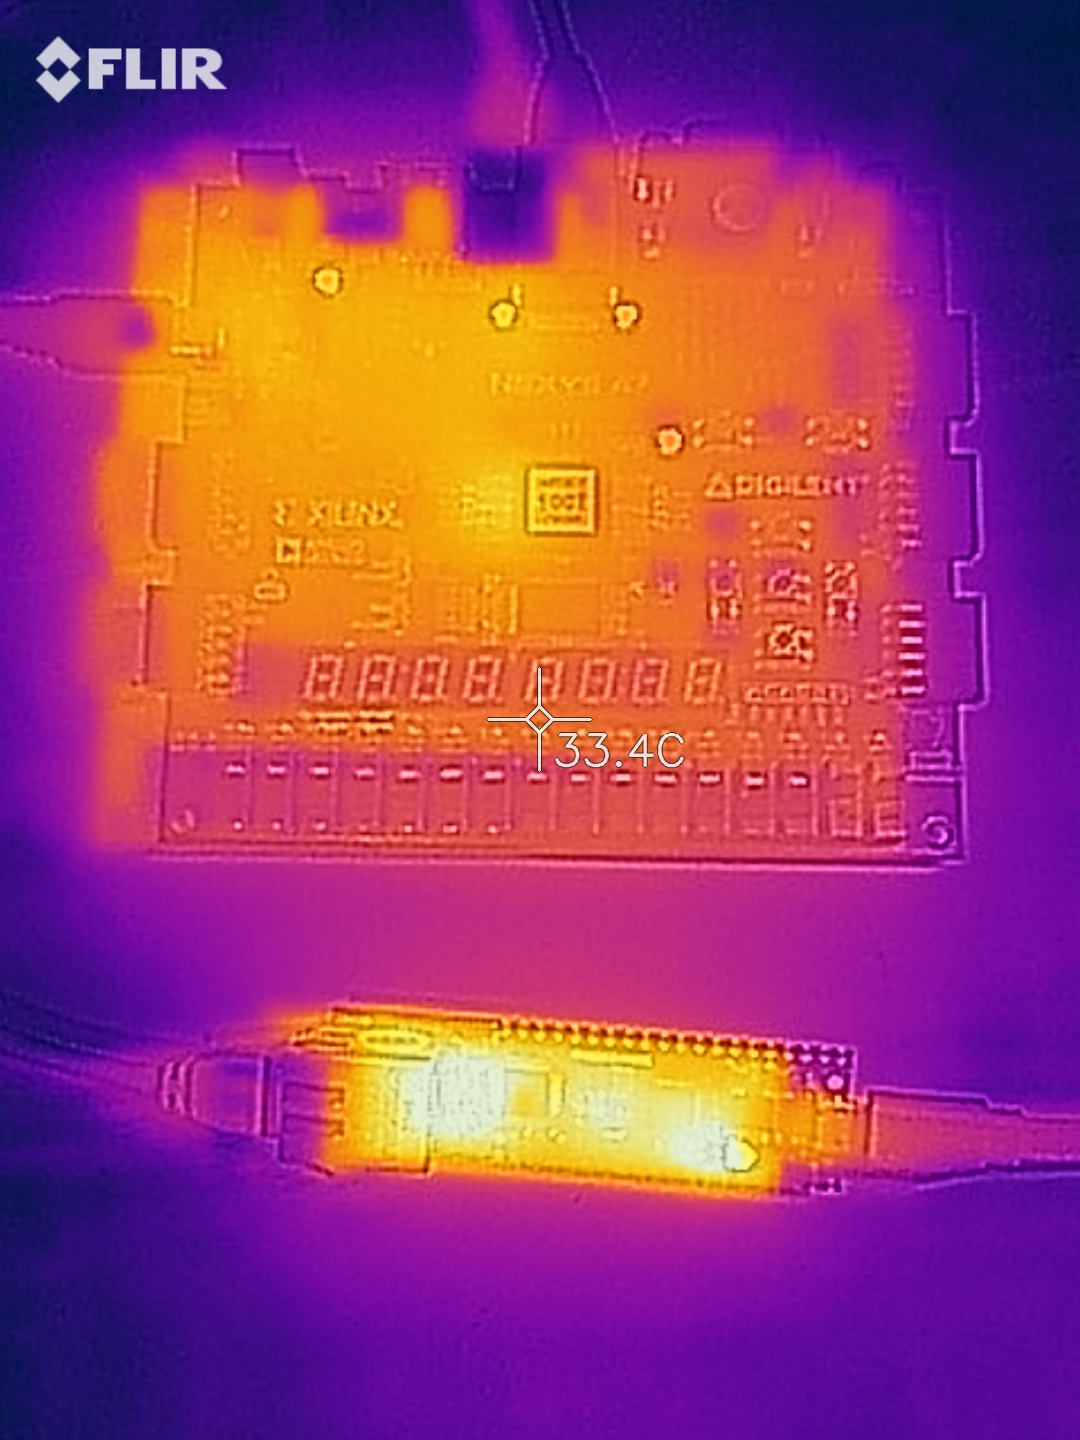
\includegraphics[width=\textwidth]{Images/flir_2hs.jpg}
        \caption{Nexys A7 (top) and WIZ5500 Pico (bottom)}
        \label{fig:thermal_2hr_fpga_pico}
    \end{subfigure}
    \hfill % this will add a small space between the two images
    \begin{subfigure}[b]{0.45\textwidth} % Adjust the width to your needs
        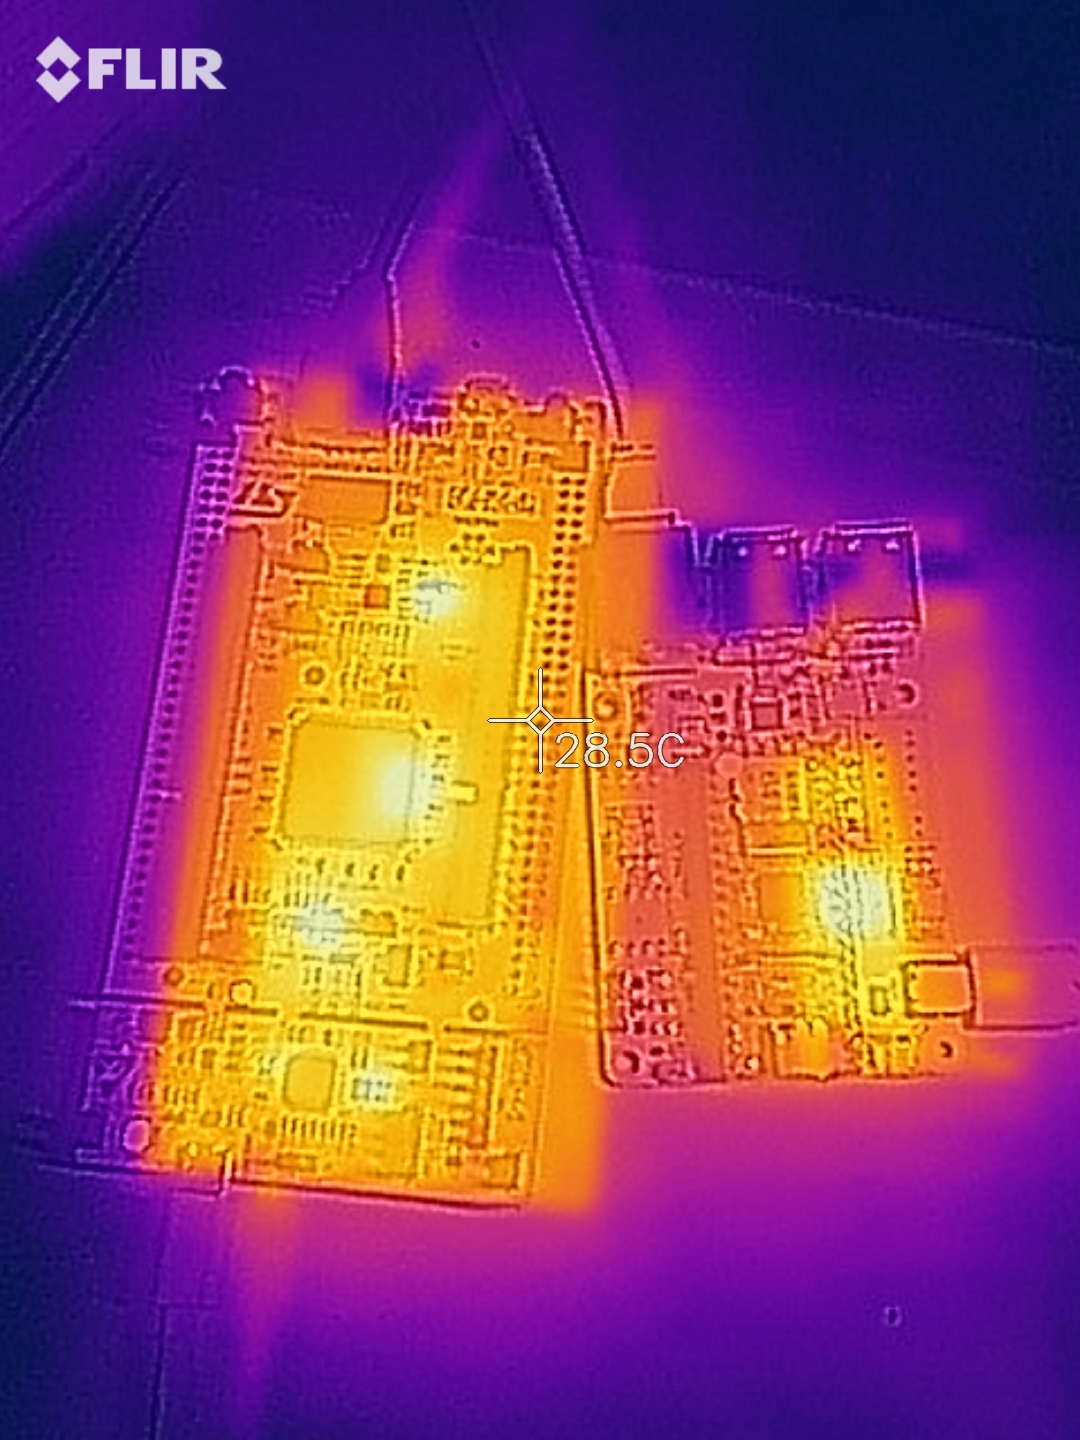
\includegraphics[width=\textwidth]{Images/flir_nucleo_milkv.jpg}
        \caption{Nucleo board (left) and MilkV Duo (right)}
        \label{fig:thermal_2hr_nucleo_milkv}
    \end{subfigure}
    \caption{Thermal images of boards under test after two hours}
    \label{fig:thermal_2hr}
\end{figure}



From figure \ref{fig:thermal_2hr_fpga_pico}, the Nexys A7 exhibits additional hotspots besides the FPGA itself, likely indicating that other components are contributing to the elevated quiescent current noted earlier. When compared with other designs, the Nexys A7 FPGA shows minimal heat output, indicating a more efficient design. However, it is important to consider the physical dimensions of the chips and their respective thermal masses.

Among the evaluated boards, the WIZ5500 exhibited the highest temperature, while the MilkV board demonstrated the lowest heat emission. The larger F767ZI board displayed a comparatively lower temperature despite having a much larger footprint and an extra PHY chip contributing to its overall heat output. In contrast, the MilkV incorporates an MCU, Ethernet MAC, and PHY within the same package. These observations indicate that WIZ5500 may not be the optimal choice for thermally sensitive applications such as recording room temperatures. Alternatives like the MilkV or an FPGA on a more efficient board with a design similar to the one created in this thesis may be more suitable.

Although these thermal measurements do not provide a great deal of useful information, they help indicate that the Nexys A7's significant power draw is not predominantly attributed to the FPGA itself and instead showcases the device's relative efficiency. The following section delves deeper into the power consumption of the design.




















\section{Power analysis}
\label{sec:power_analysis}

\subsection{Theoretical power analysis}

In this section, the power consumption of the design is analysed theoretically using Xilinx Vivado's post-synthesis power analysis summary. The findings from this summary provide useful insights into the design. However, it is important to note that these results are dependent on many variables and should only be considered as an indication of the design's power consumption.

The design's total power consumption was calculated to be 487mW, as shown in figure \ref{fig:post_synth_power_summary}. A large portion of this, 383mW, is attributed to dynamic power, which fluctuates depending on the current state and operations of the design.


\begin{figure}[h]
    \centering
    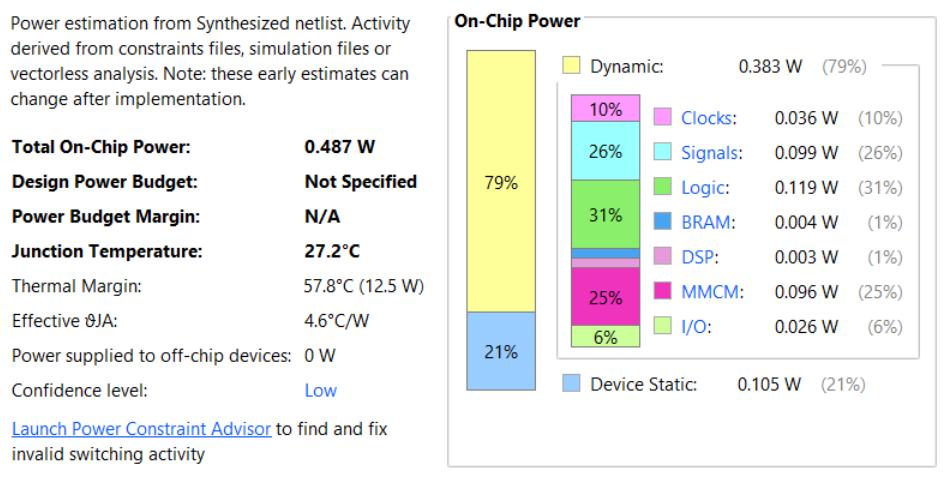
\includegraphics[width=0.75\textwidth]{Images/power_summary.png}
    \caption[Post synthesis power summary for design]{Post synthesis power summary for design.}
    \label{fig:post_synth_power_summary}
\end{figure}


Vivado further breaks down the design's power consumption into the different hierarchical components, as shown in table \ref{tab:power_consumption}. Notably, the RISC-V processor (NEORV32) constitutes to the majority of the power consumption in the design. In contrast, the Ethernet hardware consumes under 100mW while the packet classifier consumes just 2mW. This implies that incorporating a packet classifier into a design comes at a minimal power cost, making it ideal to be included in low power systems. 


\begin{table}[h]
    \centering
    \caption{Power consumption of components.}
    \begin{tabular}{lc}
        \toprule
        Name & Total (mW) \\
        \midrule
        neorv32 & 158 \\
        clk control & 97 \\
        ethernet\_mac & 97 \\
        packet classifier & 2 \\
        \bottomrule
    \end{tabular}
    \label{tab:power_consumption}
\end{table}



\subsection{Measured power analysis}

For the empirical analysis, the current was measured since the voltage remained constant across devices (5V from USB power). The Nordic Semiconductor PPK2, used for current measurements, can record up to 100kSa/s. However, a 10kSa/s sampling rate was chosen to reduce noise in the results. It's important to treat these results as indication of power consumption as they do not account for regulator inefficiencies and do not give a true power rating of the core parts of the design. 

As a baseline, the Nexys A7 board with no design loaded drew 200mA (1W at 5V), which is attributable to all the board's additional components. Upon loading the hardware design (not including the firmware), the current consumption increased to 284.4mA. After flashing the firmware, the idle current reached an average of 301.84mA, or a power draw of 1.51W was observed. Deducting the quiescent current of the board's miscellaneous components (assumed to be the baseline 200mA measurement) yields a power consumption of 0.51W,roughly aligning with the synthesis tool's calculations.

A series of tests were conducted including sending ICMP pings and web requests. When the device was pinged at 50ms intervals, the average current of 300.72mA was measured. Interestingly, the current consumption patterns were cyclic in nature, as illustrated in figure \ref{fig:ppk_icmp_ping}. Subsequent UDP ping tests resulted in a similar waveform pattern, with an average current draw of 301.13mA.

This phenomenon was explored further by blocking the network packets using the packet filter. The results revealed that the filter had a negligible impact on the current consumption, with an average current of 300.92mA. Notably, the cycle's periodicity, approximately 83ms which not only exceeds to the 50ms time between pings, but is also consistent with the previous tests, indicating that it's not a consequence of the firmware. Secondary observations were made by capturing the PHY status LED at 240 frames per second which revealed a 20-frame period (approximately 84ms), consistent with the current measurements indicating that the difference in current is due to the LED.


\begin{figure}[h]
    \centering
    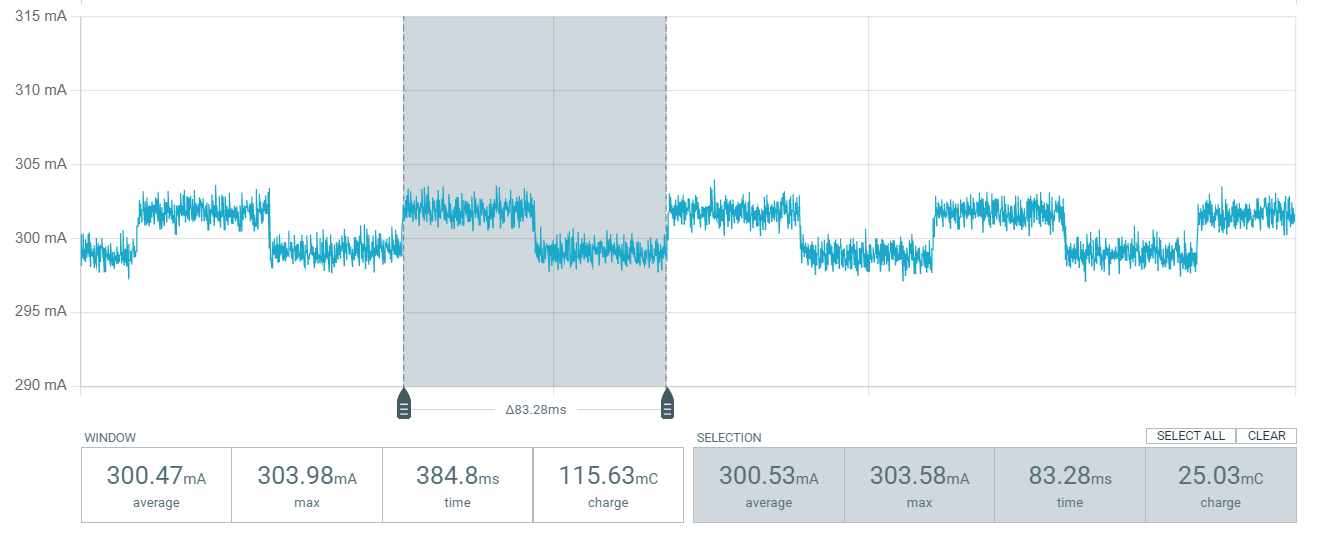
\includegraphics[width=0.9\textwidth]{Images/PPK_ping_zoom.png}
    \caption[Zoomed in current consumption for ICMP pings]{Zoomed in current consumption for ICMP pings.}
    \label{fig:ppk_icmp_ping}
\end{figure}

The subsequent test was centred around accessing the webserver, and the results are detailed in figure \ref{fig:ppk_http_annotated}, where five distinctive regions are depicted, each corresponding to a specific action.



\begin{figure}[h]
    \centering
    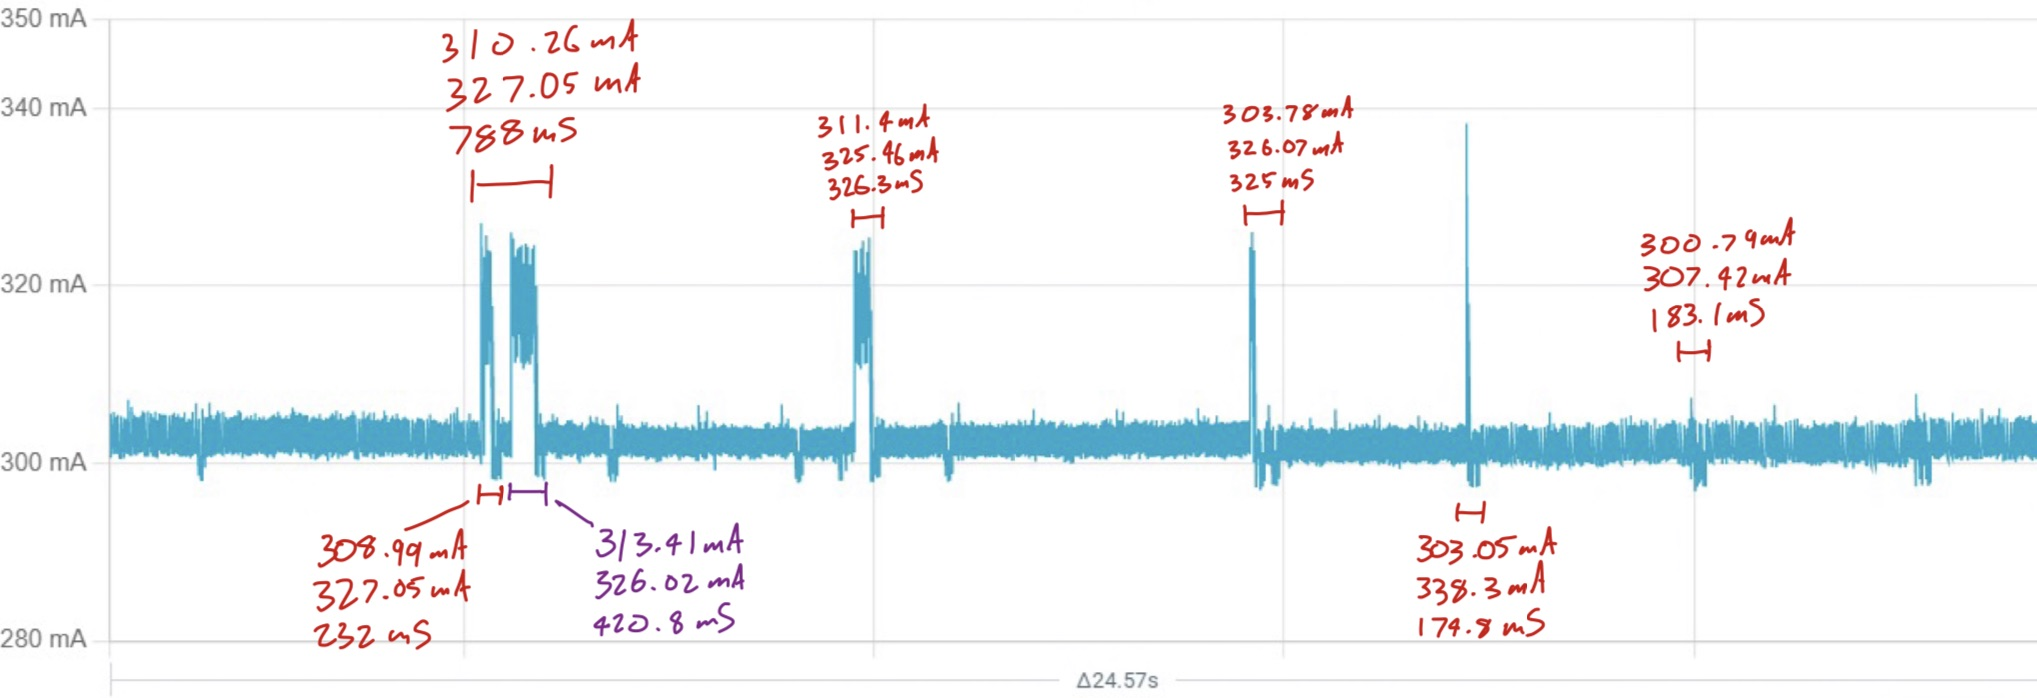
\includegraphics[width=0.9\textwidth]{Images/PPK_http_annotated.png}
    \caption[Current consumption of Nexys A7 with HTTP requests]{Current consumption of Nexys A7 with HTTP requests.}
    \label{fig:ppk_http_annotated}
\end{figure}


The first action (on the far left) is the initial HTTP GET requests. Notably, this section is split in two, as the client fetches the HTML, CSS, and favicon first, followed by a request for a considerably larger Javascript file. The readings for each of these points are given as: average current, maximum current, and time, going from top to bottom.

The second section was triggered by navigating to the 'about page'. The third part of the test involves navigating to the config page, while the fourth segment is initiated by pressing the 'load rules' button on the config page. The final test case is a result of refreshing the statistics on the main page.

A crucial observation to highlight is the role of client side routing and rendering, which makes subsequent full-page requests unnecessary and instead, only requires smaller API requests for data updates. The savings are two-fold due to the reduced network traffic and not requiring and SD card read or write operations, which greatly impact the current consumption. The fourth request, albeit involving an SD card read, is limited to accessing a single page due to the small file it is accessing. Conversely, the fifth request does not include SD card read/write operations, instead only a single SPI transaction, which consequently consumes significantly less power.

An essential learning from this is the efficacy of static page applications with client-side routing, like those created with Vue.js, in embedded systems for minimising resource utilisation, network traffic and power consumption. Another result from these tests is the negligible impact of the packet filter on the power consumption, which is Vivado predicted, making it a perfect addition to future microprocessors with built-in Ethernet MACs.
